\documentclass[../thesis.tex]{subfiles}
\graphicspath{{\subfix{figs/}}}
\begin{document}

\chapter{Methodology}
\label{ch:methods}

% start with recap of previous chapters, into: ok so now what tools can we use. start with "old" way: classic linguistics, transition into computational and finish with complex systems stuff.
% \cite{NguyenComputationalSociolinguistics2016} 

% different media to convey language
% HERE written language exclusively, WHY: our methods, because that's what computers process better
% SO we lose a lot of things that cannot be transcribed, or that are simply not because it would require considerable effort to do so  (accent, intonation), and access to spoken language is much more limited. also lose all non-verbal communication between human


% Enormous amount of information exchanged through language. Data and metadata: . Someone's language tells a lot about them

% methods with books "older data"

% data can say if model is wrong, but not if it's a good one: machine scientist stuff

\section{Data}

\subsection{What for}

\subsection{Traditional sources in linguistics}

\subsection{New sources from online media}

\subsection{The case of Twitter}

The biggest source of data we have used throughout this thesis is Twitter. Twitter is a microblogging website where people can register to share and view short posts called Tweets. These can be of three kinds:
\begin{itemize}
  \item a simple post that appears on the user profile and is shown on the homepage of
  all the users following this user, which is what people generally refer to with the
  term \emph{Tweet};
  \item a reply to another post, which can be seen by anyone but only shown on the
  homepage of the users involved in the conversation;
  \item a repost to one's profile, to share a Tweet that is already posted (which can be
  one's own), called \ac{RT};
  \item a retweet but with some added text commenting on the quoted post, called
  \ac{QRT}.
\end{itemize}
The platform is called a \emph{micro}blogging website because these posts cannot exceed 280 characters (140 before 2017). % TODO more


\subsubsection{Accessing the data}
A major advantage of Twitter for academic research is how open the platform is to giving
access to its data to researchers. One can send automatic queries to Twitter for data
through their public \ac{API} \cite{TwitterAPI}. In these queries one can specify rules
to, for instance, retrieve all the Tweets posted in a given country, in a given time
period, or which contain some given text. All the Twitter data we have used throughout
this thesis was retrieved from the filtered stream endpoint of the Twitter \ac{API}
\cite{TwitterAPIa}. We show in \cref{fig:tweet_data} an example of the data we can have
for each Tweet.

\captionsetup[subfigure]{position=top, labelfont=it,textfont=normalfont,singlelinecheck=off,justification=raggedright}
\begin{figure}
  \centering
  % \subfloat{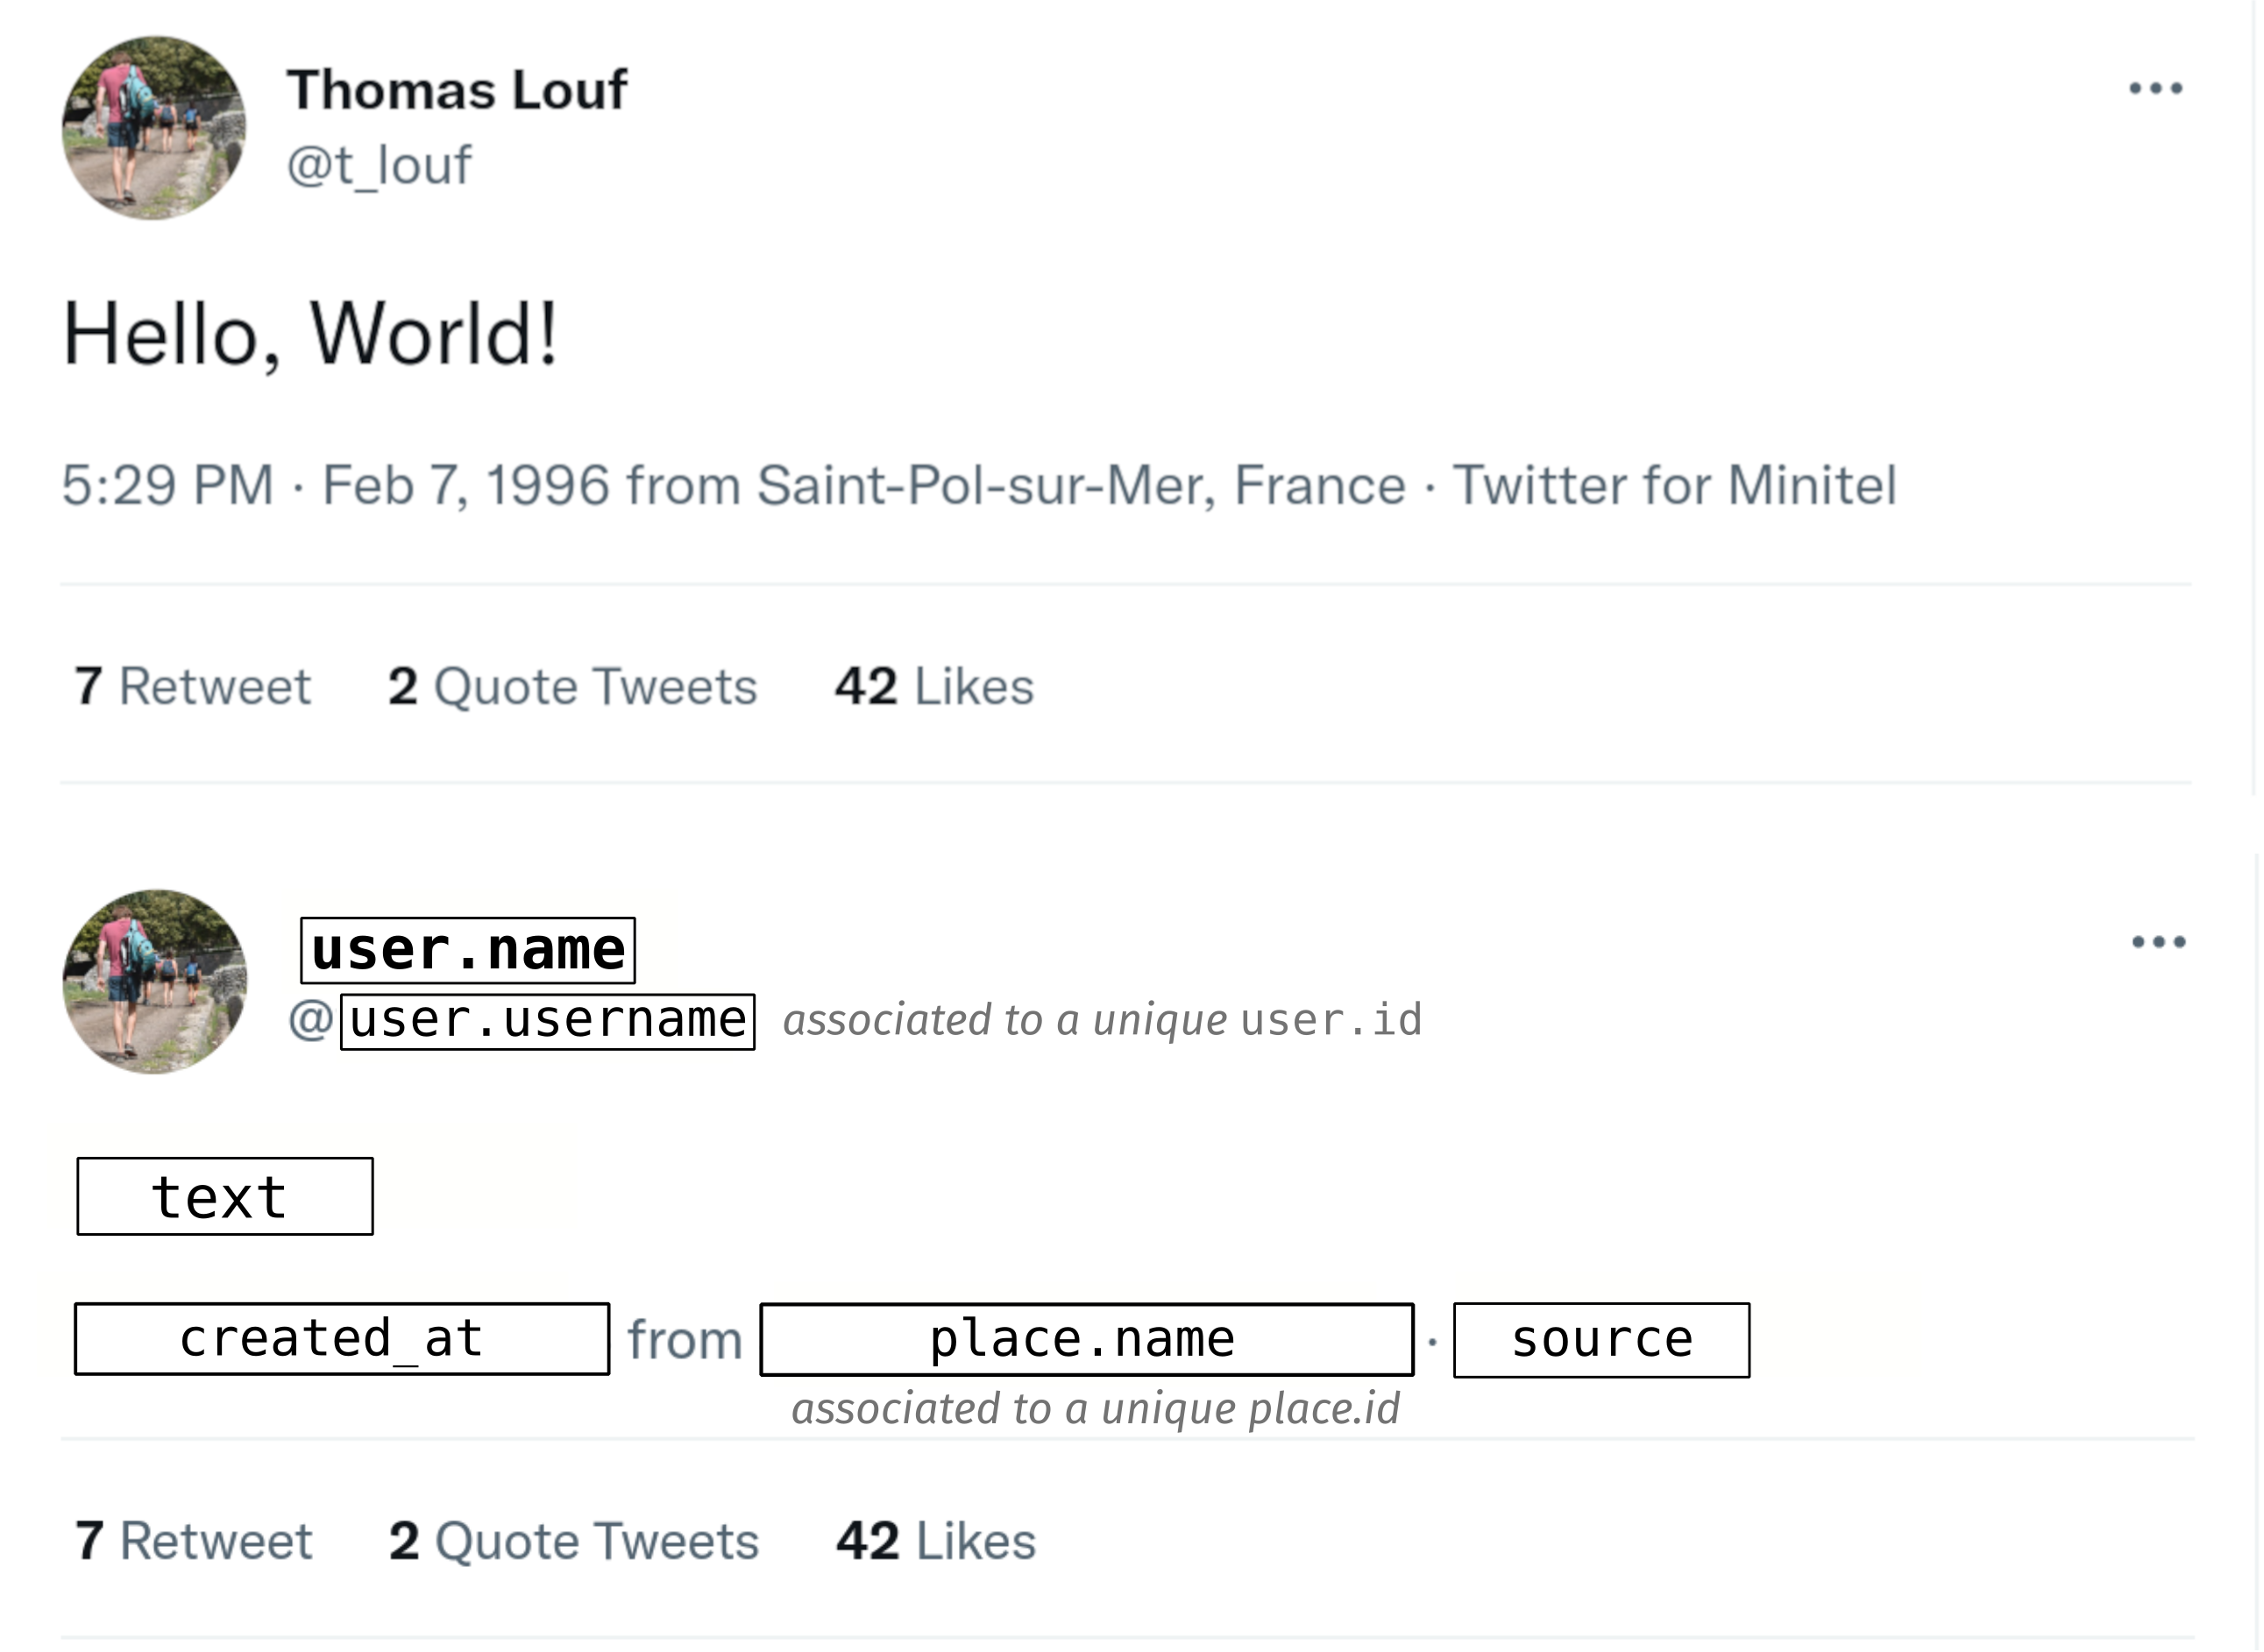
\includegraphics[width=1\textwidth]{tweet_fields.png}}
  \subfloat[][]{
    \label{subfig:tweet}
    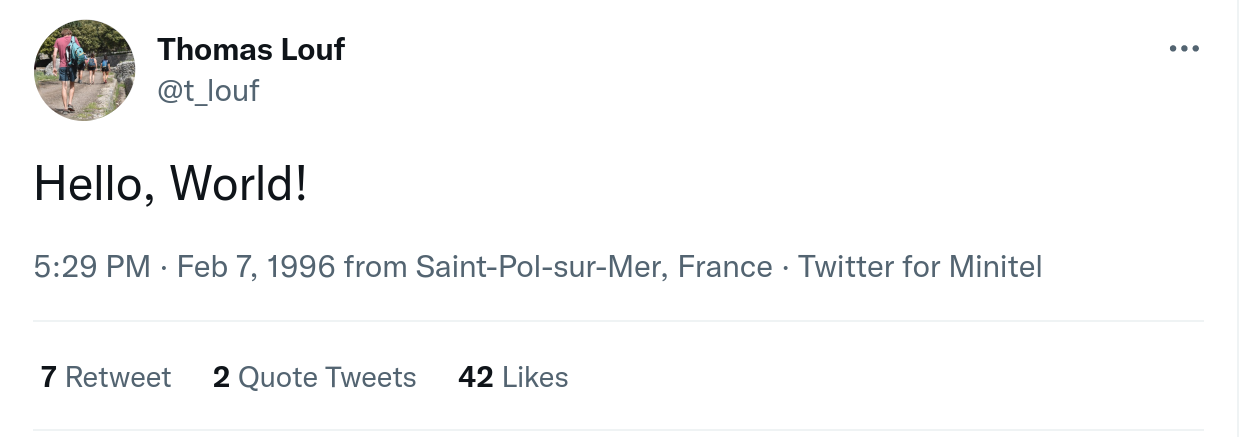
\includegraphics[width=0.95\textwidth]{tweet.png}}
  \\
  \subfloat[][]{
    \label{subfig:annotated_tweet}
  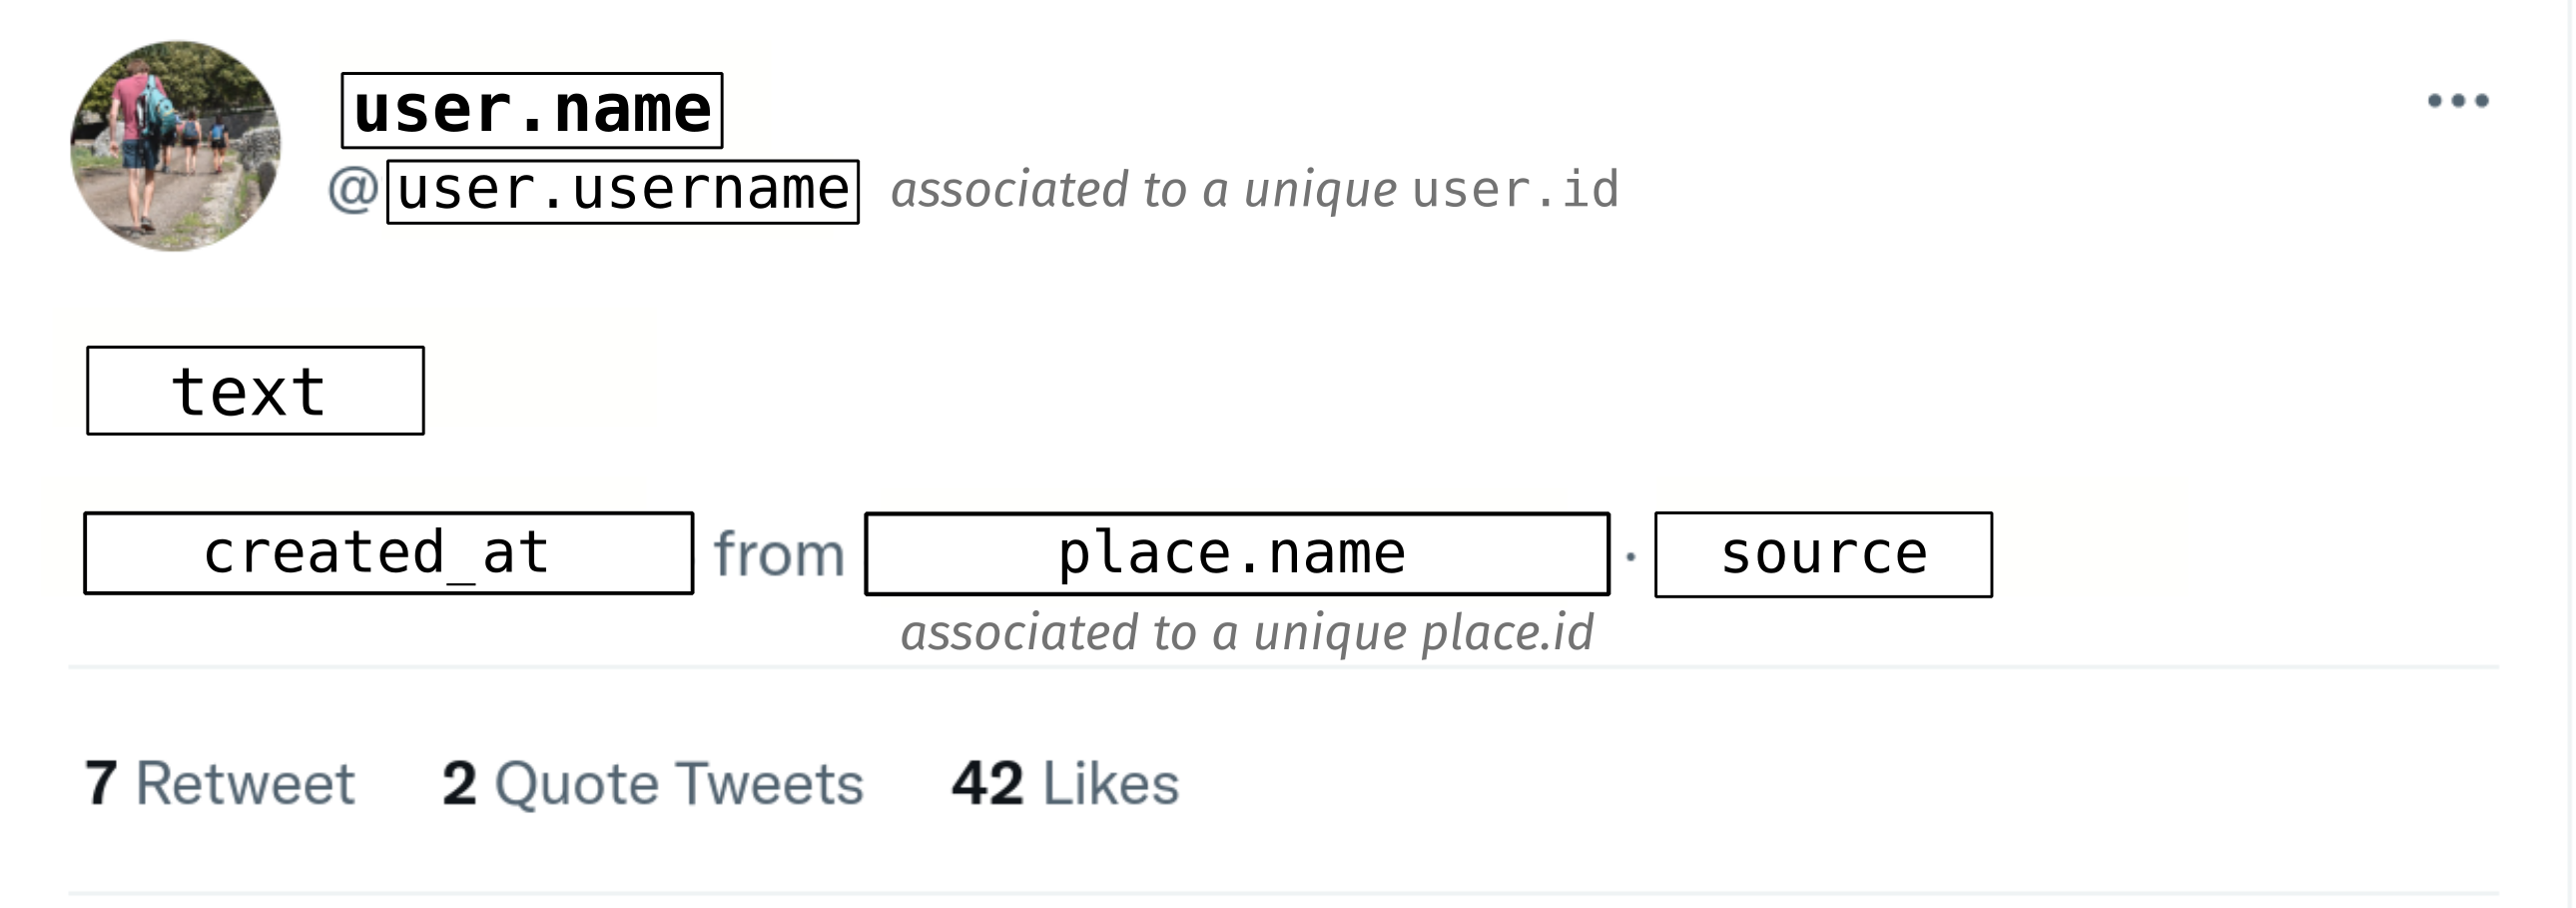
\includegraphics[width=0.95\textwidth]{annotated_tweet.png}}
  \\
  \begin{SubFloat}{\label{subfig:json}}
    \begin{minipage}[b]{0.95\linewidth}
      \begin{verbatim}
        {
          "id": "1234567890",
          "text": "Hello, World!",
          "created_at": "1996-02-07T04:29:05.000Z",
          "geo": {
            "place_id": "f68f3d5396bd681c",
            "coordinates": {
              "type": "Point",
              "coordinates": "[2.3295, 51.0249]"
            }
          },
          "source": "Twitter for Minitel",
          "user": {
            "id": "123",
            "username": "t_louf",
            "name": "Thomas Louf"
          }
        }
      \end{verbatim}
    \end{minipage}
  \end{SubFloat}
  \caption[]{A Tweet data. We show \subref{subfig:tweet} an example Tweet as displayed
  on Twitter and \subref{subfig:annotated_tweet} a version annotated with the name of the
  fields in \subref{subfig:json} the data as it would be sent by the \ac{API}, which is
  simply text formatted in a dictionary-like structure (JSON).}
  \label{fig:tweet_data}
\end{figure}

There are two fields in these data that particularly interest us for the works we will
present in the next part and that need careful processing: the textual content of the
Tweet (in \texttt{text}) and its geotag (in \texttt{geo}). Next, we detail the usual
steps we take to process these. 


\subsubsection{Text processing}
\label{sec:method_text_process}
Since we are interested in the speech produced by users, we need to clean parts of the
text which cannot be considered as natural language production. Those are the URLs,
mentions of other users (in the form \texttt{@username}) and hashtags (in the form
\texttt{\#topic}). It is not completely obvious that the latter should be discarded
though. Hashtags are used on Twitter to aggregate Tweets by topics. It is an important
feature of the website, whose aim is to enable users to easily find the Tweets of other
users discussing similar topics, inversely to make one's Tweets more discoverable by
others, and to see real time trends on the platform. Hence, there can be completely
different motivations behind writing a hashtag: to actually tag a Tweet with one or more
topic, to promote the Tweet, or simply follow a trend. Thus, the content of hashtags can
deviate significantly from normal speech \cite{PageLinguisticsSelfbranding2012}. It is
therefore safer to discard hashtags entirely, which is no issue as long as we can
collect enough textual content without them anyway. We actually made some measurements
in our Tweets' database to see if that was the case. We took several random samples of a
million Tweets each, stripped them of URLs and mentions, and then computed the ratio of
characters within a hashtag compared to the total number of characters left in those
Tweets. This proportion was found to be consistently below \SI{5}{\percent}. We thus
consider the precaution of stripping hashtags off of Tweets worth taking. One last kind
of element that we discard are source-dependent. We will not go into details --- our
text processing code is freely available online anyway --- but, for instance, when a
Tweet was sent from Foursquare, we strip all location-related content, which can be
located after either a \texttt{``I'm at''} or \texttt{``( @ ''} string.

In practice, all the elements cited above are stripped off of Tweets using regular
expressions. After this cleaning step, for what follows we then keep only the Tweets
still containing at least four words. The next important step that was crucial to all
our works was to infer the language the Tweets are written in. To do so, we leverage a
trained neural network model for language identification: the Compact Language Detector
\cite{SalcianuCompactLanguage2023}. It was designed as part of Chromium-based web
browsers to detect the language web pages are written in in order to make translation
suggestions to users, and it is now openly accessible. Its output is a language
prediction along with the confidence of the model. Whenever we focus on a language, we
thus keep Tweets which are tagged in that language with a confidence above
\SI{90}{\percent}.

We have thus described the basic steps of text pre-processing that are recurrent in our
works. Out of it we get the Tweets for which we could reliably assign a language,
stripped of the parts which are irrelevant to us.


\subsubsection{Inferring geolocation}
\label{sec:method_geoloc}
The steps presented above allow us to measure linguistic features of interest from our
Tweets. A next step we usually take is to map those measurements geographically. We are
able to do so thanks to the information contained in the \texttt{"geo"} field of a
Tweet, an example of which is shown in \cref{fig:tweet_data}. This example is actually a
particular case, because of the presence of the \texttt{"coordinates"} field. This gives
precise GPS coordinates of the location of the device used to send out the Tweet: a
longitude, latitude pair. It is present in a Tweet's metadata when the device's GPS is
enabled \emph{and} when the user opted in for precise location tagging in the parameters
of the application. As this setting is opt-in (so off by default), very few users
actually have this enabled: from our measurements, roughly between $10$ and
\SI{20}{\percent} of those who posted with their GPS enabled between 2015 and 2019,
depending on the country. This setting has been in place since 2015, which is the
starting year of the datasets we have used throughout this thesis. So when a user
enables their device's GPS with precise geolocation disabled and this
\texttt{"coordinates"} field is absent, how do we infer geolocation? In this majority
case, the geotag we have is the \texttt{"place\_id"} we show in the example. This
identifies a place: a specific, named location, which can be of different scales:
\begin{itemize}
    \item a country,
    \item an administrative unit: province, region or department for instance,
    \item a city,
    \item a \ac{POI}: any kind of public place: restaurant, school, event venue, etc.
    These are represented by a point, so Tweets tagged with a \ac{POI} can be considered
    similarly to the ones with coordinates.
\end{itemize}
When a user tweets with their device's GPS activated, a place (usually the city they
tweet from) is selected by default, and they can switch to another one from a list of
close-by places. These places were fed to Twitter by Foursquare
\cite{FoursquarePlaces2019} (among others), which provides data down to a \ac{POI} level
for more than 190 countries. The geographical extent of places other than \acp{POI} is
defined by bounding boxes.

To map linguistic features, Tweets must be attributed to the geographical areas of
interest of the study. These may be defined by administrative boundaries (US counties,
for example) or by us (a regular grid of cells of equal area, for instance). As ``area''
is an ambiguous term that can also refer to the measure of the size of a surface, in the
following we will refer to these areas only by the term \emph{cells}. So, when a Tweet
has GPS coordinates or a \ac{POI} as a geotag, the attribution is straightforward: there
can be only one matching cell. When it has a place defined by a bounding box, it is not
so trivial. The naive approach would be to take the centroid of the place and attribute
to the cell containing it. This is problematic, though. As the cells to match are not
necessarily regular, this method does not systematically match the place to the cell
with the most overlap. A less naive approach would then consist in computing the area of
overlap for every candidate cell and match to the one with biggest such area. This would
still be an all-or-nothing attribution though. What if the place has \SI{51}{\percent}
of its area in one cell and \SI{49}{\percent} in another? It would not be reasonable to
attribute that Tweet to the first cell only. To account for the uncertainty we have when
doing this cell matching, we thus rather do a partial attribution. We attribute the
Tweet to possibly more than one cell, with ratios defined by the ones of the place's
area that lies within each cell. For the example above, and when computing a basic
metric like a count, this means that we attribute \SI{51}{\percent} of the count to one
cell and \SI{49}{\percent} to the other. Because the scales of places span orders of
magnitude, some may intersect many cells. There can then be so much uncertainty in the
actual geographic origin of the Tweet that it is preferable to discard it. Our criterion
here is that when the four cells which contain most of the place's area put together do
not contain more than \SI{90}{\percent} of its total area, the place, and all the Tweets
assigned to it, are discarded. 

As the activity of Twitter users was found to follow a log-normal distribution spanning
almost four orders of magnitude \cite{MocanuTwitterBabel2013}, it can be preferable to
compute metrics at the user level. Indeed, at the Tweet level, the linguistic behaviour
of the most active users could overshadow the one of the many, less active users.
Individuals are mobile but for the vast majority they have a preferred location, namely
their place of residence. That is why we often strive to attribute a cell of residence
to the users in our datasets. To explain the heuristics we defined for residence
attribution, let us first formalize some notation. For each user $u$, there are two
counts we get directly from their Tweets: the number of them with GPS coordinates that
fall in cell $c$: $n_{u, c}^{\text{GPS}}$, and those without coordinates but tagged as
being from place $p$: $n_{u, p}$.  We wish to compute $r_{u, c} \in \mathbb{R}^+$, the
ratio of Tweets of user $u$ in cell $c$. It can be decomposed into the contributions of
those with GPS coordinates $r_{u, c}^{\text{GPS}}$, and of the others: $r_{u,
c}^{\text{P}}$:
\begin{equation}
  r_{u, c}
    = r_{u, c}^{\text{GPS}} + r_{u, c}^{\text{P}}
    = n_{u, c}^{\text{GPS}} + r_{u, c}^{\text{P}}.
\end{equation}
Denoting $A_p$ and $A_{p \cap c}$ the areas of the place $p$ and of the intersection
between $p$ and $c$, respectively, the partial attribution described above yields:
\begin{equation}
  r_{u, c} = n_{u, c}^{\text{GPS}} + \sum_p n_{u, p} \frac{A_{p \cap c}}{A_p}.
\end{equation}
To attribute a cell of residence to each user $u$, we first only consider cells where
$r_{u, c} \geq 3$ and $r_{u, c} / \sum_{c'} r_{u, c'} \geq 0.1$. We also compute
$r_{u,c}$ considering only Tweets posted at nighttime (from 6pm to 8am), that we denote
$r_{u, c}^\text{NT}$. Among those left, the cell of residence $c^*$ is then the one
such that $r_{u, c^*}^\text{NT} / \sum_{c'} r_{u, c'}^\text{NT} \geq 0.5$, if any. This
roughly means that we impose that a user must have tweeted at least three times and at
least \SI{10}{\percent} of the time from that cell, and that at night the majority of
their Tweets were from there. All users for whom a cell of residence cannot be
attributed are subsequently discarded from the analysis. All three thresholds may be
adjusted to each analysis, and also tweaked for sensitivity analyses.  


% TODO: rearrange to make this first pre-processing subsubsec? since it's the one done
% first chronologically / at same time to compute movespeed between consecutive tweets
% you need to understand what geotags are...
\subsubsection{Selecting relevant users}
\label{sec:method_users_select}
As we are interested in the natural speech produced by individuals, we start our
analyses by filtering out users whose behaviour resembles that of a bot. We first
eliminate those tweeting at an inhuman rate, set at an average of ten tweets per hour
over their whole tweeting period. Then, we only keep those who tweeted either from a
Twitter official app, Instagram, Foursquare or Tweetbot (a popular third-party app).
These were selected because they are significantly popular among real users. Also,
consecutive geolocations implying speeds higher than a plane's (\SI{1000}{\kilo \meter
\per \hour}) are detected to discard users. The final filter is optional: when we wish
to only keep residents of the region considered, we impose for a user to have tweeted
from there in at least three consecutive months.


\subsubsection{Caveats}
No data source is without bias, and Twitter is no exception.
% cover Twitter (biases but also basic technical details, API, what Tweet looks like), why remove HTs, blabla, language IDtion data driven analysis, cite Bruno papers eg

% theoretical models: AS, MW 

% finally computational methods, very general (data, PCA...)


\section{Models}

\subsection{What for}

\subsection{What kind}

\ac{ABM}


\section{Source materials and tools}
Following the principles of open science, throughout my thesis, I have made all source
materials for my results openly accessible, whether they are codes\footnote{Hosted on
GitHub at \url{https://github.com/TLouf}} or datasets\footnote{Hosted on figshare at
\url{https://figshare.com/authors/Thomas_Louf/9441395}}, including this very
manuscript's\footnote{Hosted at \url{https://github.com/TLouf/phd-thesis}}. Equally importantly, I believe, I have strived to use almost exclusively free
and open source software in my work. I cannot realistically cite here all projects I
have relied on to carry out my work, but I can cite a few central ones. I wrote all my
code in the Python 3 programming language, using libraries such as
NumPy~\cite{HarrisArrayProgramming2020},
pandas~\cite{teamPandasdevPandas2020} or
GeoPandas~\cite{JordahlGeopandasGeopandas2020}. In their vast majority, figures
presented here were prepared with Matplotlib~\cite{HunterMatplotlib2D2007}, and
sometimes edited, or entirely drawn, with Inkscape\footnote{Available at
\url{https://inkscape.org}}.

This document was prepared using \LaTeX\ with the \texttt{classicthesis}
style\footnote{Hosted at \url{https://www.ctan.org/pkg/classicthesis}} developed by
Andr\'e Miede and Ivo Pletikosić, and the LaTeX Workshop extension\footnote{Hosted at
\url{https://github.com/James-Yu/LaTeX-Workshop}} of Visual Studio Code.
% managed the references cited in this work with Zotero https://www.zotero.org/


\section{Outline}



\end{document}
